\chapter{Mengenal Kecerdasan Buatan dan Scikit-Learn}

\section{Teori}
Praktek teori penunjang yang dikerjakan :
\begin{enumerate}
	\item Sejarah Dalam Perkembangan \textit{Artifical Intelligence}. \textit Teknologi kecerdasan buatan atau yang dikenal dengan AI (artificial intelligence), disadari atau tidak, telah menjadi bagian tak terpisahkan dari kehidupan kita. Setiap kata yang kami ketik di mesin pencari, setiap percakapan yang kami kirim ke teman kami, setiap foto yang kami unggah ke jejaring sosial, setiap rupee yang kami transfer ke akun lain; semua ini tersentuh oleh AI.
	
	Namun, hal ini tidak selalu terjadi. Ratusan tahun yang lalu, AI hanya hidup di benak para filsuf. Padahal, puluhan tahun  lalu, AI masih sebatas tulisan para ahli komputer. Sekarang, dunia akan berada dalam kekacauan total jika AI tiba-tiba menghilang. Untuk memahami secara umum bagaimana AI dapat berkembang begitu cepat, dari konsep untuk filsuf hingga bantuan bagi semua orang, kita perlu melihat sejarah.\\
	Pada akhir tahun 1950 \textit merupakan masa aktifnya usaha di bidang AI. Program kerja AI pertama  ditulis pada tahun 1951 untuk menjalankan mesin Ferranti Mark I di University of Manchester (UK):  program permainan bernaskah yang ditulis oleh Christopher Strachey dan program permainan catur yang ditulis oleh Dietrich Prinz. John McCarthy menciptakan istilah "kecerdasan buatan" pada konferensi pertama yang membahas topik tersebut, pada tahun 1956. Dia juga penemu bahasa pemrograman Lisp. Alan Turing memperkenalkan "Tes Turing" sebagai  cara untuk menjalankan pengujian perilaku cerdas. Joseph Weizenbaum membangun ELIZA, sebuah chatterbot menggunakan psikoterapi Rogerian.
	
	
	
	Selama tahun 1960-an dan 1970-an, Joel Moses mendemonstrasikan kekuatan penalaran simbolis untuk mengintegrasikan masalah ke dalam program Macsyma, program matematika berbasis pengetahuan pertama yang berhasil. Marvin Minsky dan Seymour Papert menerbitkan Perceptrons, yang menunjukkan keterbatasan jaringan saraf sederhana, dan Alain Colmerauer mengembangkan bahasa komputer Prolog. Ted Shortliffe mendemonstrasikan kekuatan sistem berbasis aturan untuk mewakili dan menyimpulkan pengetahuan dalam diagnosis dan perawatan medis, kadang-kadang disebut sebagai sistem pakar pertama. Hans Moravec telah mengembangkan kendaraan yang dikendalikan komputer pertama untuk mengatasi rintangan kusut secara mandiri.
	
	
	\item Definisi supervised learning, klasifikasi, regresi dan unsupervised learning. Data set, training set dan testing set
	\begin{itemize}
		\item Supervised Learning
		\par
		\textit{Supervised learning}
		adalah  label di tiap data nya. Label maksudnya adalah tag dari data yang ditambahkan dalam machine learning model. Contohnya gambar kucing di tag “kucing” di tiap masing masing image kucing dan gambar anjing di tag “anjing” di tiap masing gambar anjing. Machine learning kategori dapat berupa clasification (“anjing”, “kucing”, “beruang”, dsb) dan regression ( berat badan, tinggi badan dsb). Supervised learning banyak digunakan dalam memprediksi pola dimana pola tersebut sudah ada contoh data yang lengkap, jadi pola yang terbentuk adalah hasil pembelajaran data lengkap tersebut. Tentunya jika kita memasukan data baru, setelah kita melakukan ETL (Extract Transform Load) maka kita mendapat info feature feature dari sample baru tersebut. Kemudian dari feature feature tersebut di compare dengan pattern clasification dari model yang didapat dari labeled data. Setiap label akan dicompare sampai selesai, dan yang memiliki percentage lebih banyak akan diambil sebagai prediksi akhir.
		\item Unsupervised Learning
		\par
		\textit{Unsupervised Learning} adalah sub artificial inteligence. Machine learning itu sendiri terbagi menjadi jika dikategorikan berdasarkan label. Label yang dimaksudkan disini adalah target variable ada tidak dasar datanya.
		\item Klasifikasi
		\par
		\textit{Klasifikasi} adalah sebuah proses menggunakan algoritma untuk secara akurat memasukan data kedalam kategori yang spesifik.
		\item Regresi
		\par
		\textit{Regresi} adalah Metode statistik yang digunakan dalam keuangan, investasi dan industri lainnya. Tujuannya adalah untuk mencoba menentukan kekuatan dan karakter hubungan antara  variabel dependen (biasanya dilambangkan dengan Y) dan serangkaian variabel lain (disebut variabel independen).
		\item Dataset
		\par
		\textit{Dataset} adalah suatu kumpulan data yang berisi informasi-informasi lama, dan dapat dikelola sehingga menjadi sebuah informasi baru.
		\item Training set
		\par
		\textit{Training set} adalah bagian dari kumpulan data yang kami latih untuk membuat prediksi atau menjalankan fungsi algoritme ML. Kami memberikan petunjuk melalui algoritme sehingga mesin yang kami latih dapat mencari korelasinya sendiri atau mempelajari pola dari data yang diberikan.
		\item Testing set
		\par
		\textit{Testing set} adalah bagian dari dataset yang digunakan untuk melihat tingkat keakuratan dan performa dari algoritma.
	\end{itemize}
	
\end{enumerate}


\section{Instalasi}

\begin{enumerate}
	\item Melakukan installasi pada anaconda promt dengan perintah " pip install -U scikit-learn".
	\begin{figure}[!htbp]
		\centering
		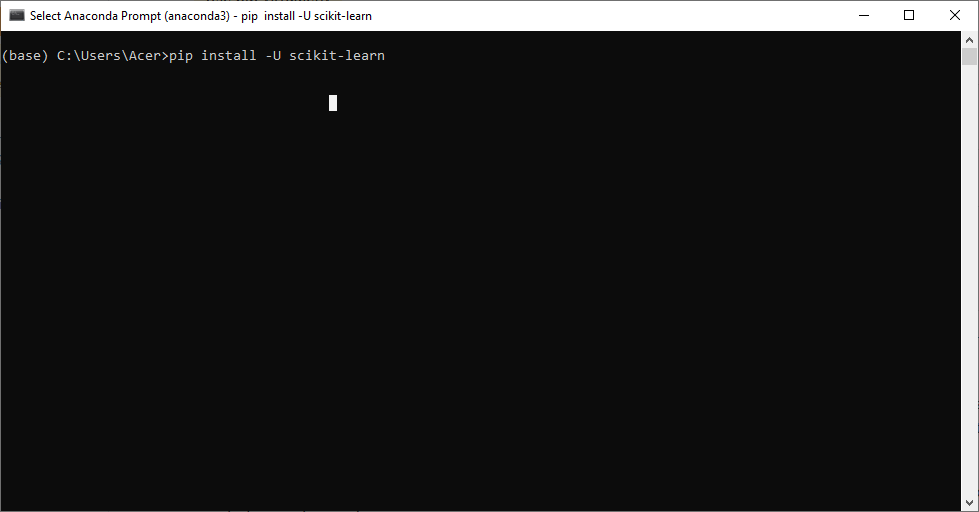
\includegraphics[scale=0.4]{figures/1.PNG}
	\end{figure}
	\newpage
	\item Kemudian klik link berikut ini untuk melakukan basic tutorial \textit{scikit-learn} "https://scikit-learn.org/stable/tutorial/basic/tutorial.html".
	\item
	Mencoba Loading an example dataset
	\begin{figure}[!htbp]
		\centering
		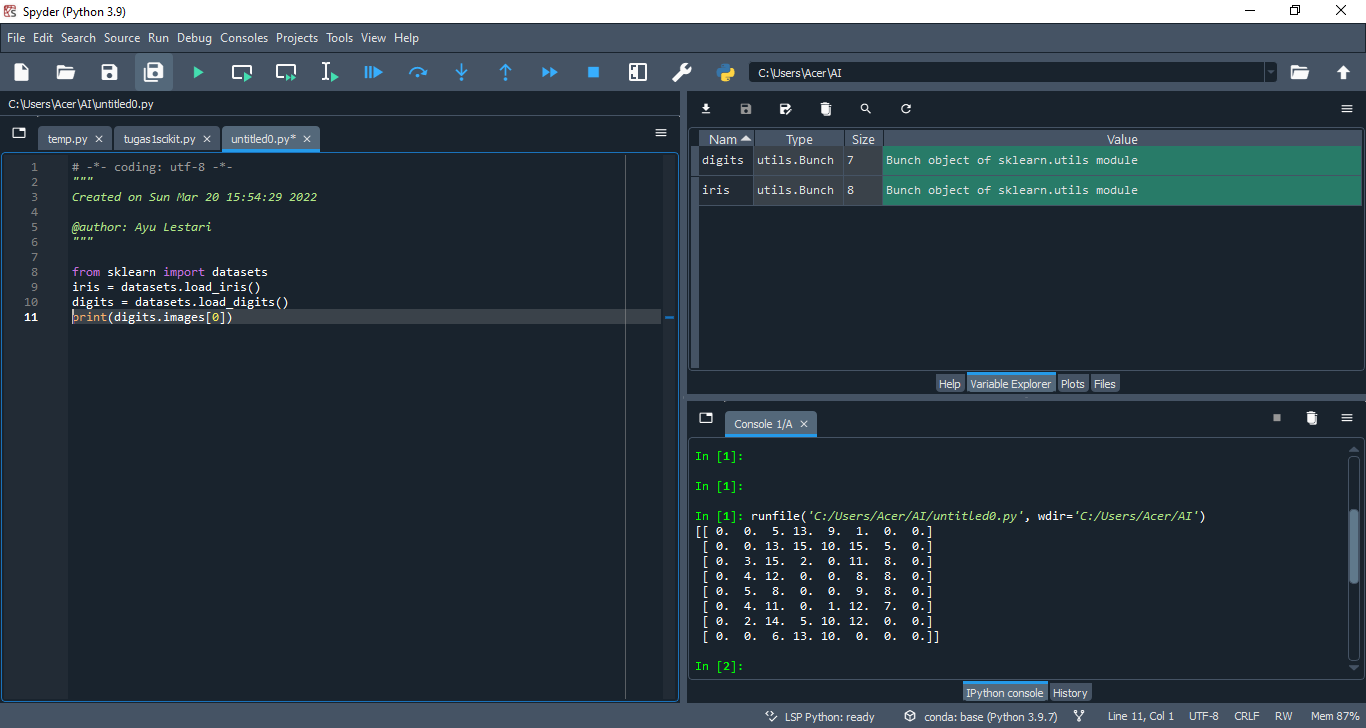
\includegraphics[scale=0.4]{figures/2.PNG}
	\end{figure}
	\item
	Mencoba Learning and predicting
	\begin{figure}[!htbp]
		\centering
		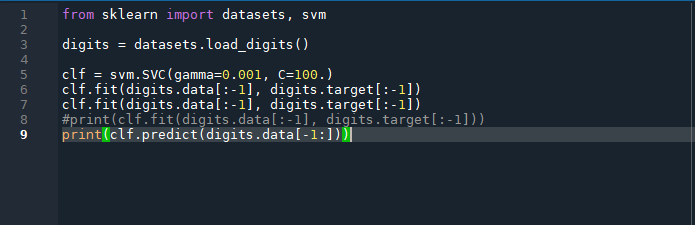
\includegraphics[scale=0.4]{figures/3.PNG}
	\end{figure}
	\newpage
	\item 
	Mencoba Conventions
	\begin{figure}[!htbp]
		\centering
		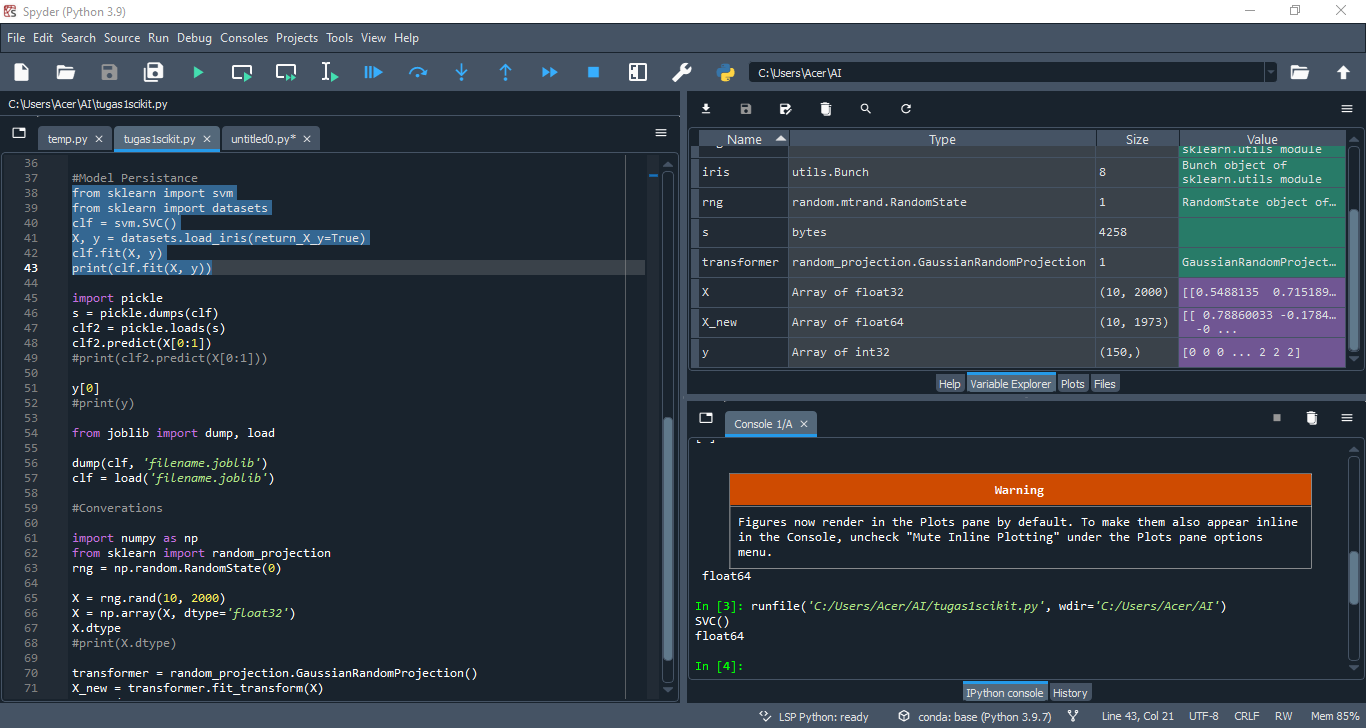
\includegraphics[scale=0.4]{figures/4.PNG}
	\end{figure}
	\newpage
	\item Link Youtube praktikum : https://youtu.be/jK0O9TWqw-0
\end{enumerate}


\section{Penanganan Error}
Dari percobaan yang dilakukan di atas, apabila mendapatkan error maka:

\begin{enumerate}
	\item Screenshoot Error
	\begin{figure}[!htbp]
		\centering
		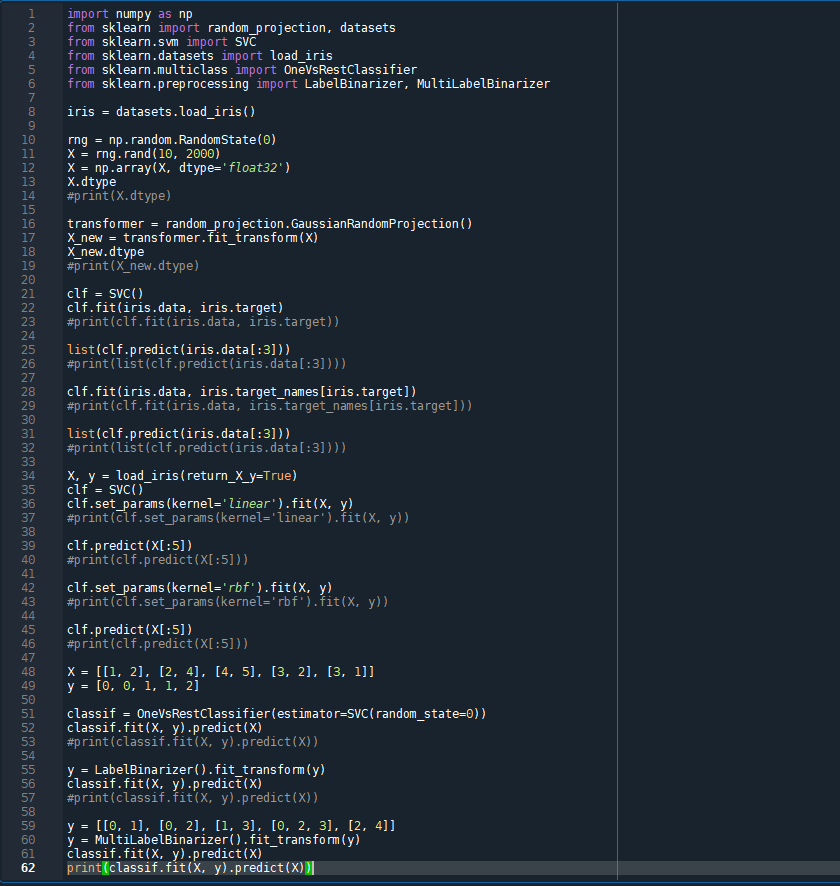
\includegraphics[scale=0.6]{figures/5.PNG}
	\end{figure}
	
	\newpage    
	\item Tuliskan kode error dan jenis error
	\par 
	Unexpected value error array
	\par

	
	\item
	Solusi pemecahan masalah error tersebut
	\par
	clf.fit digits data tidak bisa langsung di print karna masih menyesuailkan data -1. Kita bisa melakukan print pada clf.predict
	
\end{enumerate}

